\documentclass[12pt,a4paper]{article}
\usepackage{adjustbox}
\usepackage[a5paper, margin=10mm, onecolumn]{geometry}
\usepackage{tfrupee}
\usepackage{cite}
\usepackage{amsmath,amssymb,amsfonts,amsthm}
\usepackage{algorithmic}
\usepackage{graphicx}
\usepackage{textcomp}
\usepackage{xcolor}
\usepackage{listings}
\usepackage{enumitem}
\usepackage{mathtools}
\usepackage{gensymb}
\usepackage{comment}
\usepackage[breaklinks=true]{hyperref}
\usepackage{tkz-euclide}
\usepackage{array}
\usepackage{longtable}
\usepackage{calc}
\usepackage{multirow}
\usetikzlibrary{circuits.ee.IEC}
\usepackage{circuitikz}
\usepackage{hhline}
\usepackage{ifthen}
\usepackage{lscape}
\usepackage{booktabs}
\usepackage{fancyhdr}
\usepackage{float}
\usepackage{tikz}
\usetikzlibrary{positioning, shapes.geometric, arrows}

\definecolor{codegreen}{rgb}{0,0.6,0}
\definecolor{codegray}{rgb}{0.5,0.5,0.5}
\definecolor{codepurple}{rgb}{0.58,0,0.82}
\definecolor{backcolour}{rgb}{0.95,0.95,0.92}

\lstdefinestyle{mystyle}{
    backgroundcolor=\color{backcolour},   
    commentstyle=\color{codegreen},
    keywordstyle=\color{magenta},
    numberstyle=\tiny\color{codegray},
    stringstyle=\color{codepurple},
    basicstyle=\ttfamily\footnotesize,
    breakatwhitespace=false,         
    breaklines=true,                 
    captionpos=b,                    
    keepspaces=true,                 
    numbers=left,                    
    numbersep=5pt,                  
    showspaces=false,                
    showstringspaces=false,
    showtabs=false,                  
    tabsize=2
}

\lstset{style=mystyle}

\setlength{\headheight}{1cm}
\setlength{\headsep}{0mm}

\pagestyle{fancy}
\fancyhf{}
\fancyhead[L]{\leftmark}
\fancyhead[R]{\thepage}

\numberwithin{equation}{section}
\numberwithin{figure}{section}
\numberwithin{table}{section}

\title{HARDWARE ASSIGNMENT-2 }
\author{EE24BTECH11029 - SHRETHAN REDDY}
\date{\today}

\begin{document}

\maketitle

\section{Objective}
A scientific calculator is an essential tool for engineers and students, capable of performing complex mathematical operations. This project aims to develop a scientific calculator using an embedded system, specifically the Arduino Uno, programmed with AVR-GCC.

\section{System Design}
The calculator system comprises three main components:
\begin{enumerate}
    \item \textbf{Input Module}: 23-button keypad matrix
    \item \textbf{Processing Unit}: Arduino Uno (ATmega328P)
    \item \textbf{Output Module}: 16×2 LCD display
\end{enumerate}

\begin{figure}[H]
    \centering
    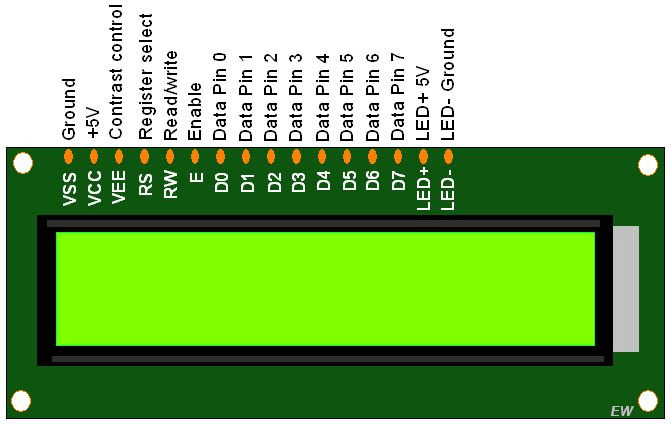
\includegraphics[width=0.8\linewidth]{figure/fig.png}
    \caption{System Block Diagram}
    \label{fig:block_diagram}
\end{figure}

\section{Hardware Implementation}

\subsection{Components Specification}
\begin{table}[H]
    \centering
    \caption{Component Specifications}
    \begin{tabular}{lll}
        \toprule
        \textbf{Component} & \textbf{Quantity} & \textbf{Specification} \\
        \midrule
        Arduino Uno & 1 & ATmega328P @ 16MHz \\
        16×2 LCD & 1 & HD44780 controller \\
        Tactile switches & 23 & 6mm×6mm \\
        Resistors & 3 & $1k\Omega$ (2), $1.5k\Omega$ (1) \\
        Breadboard & 2 & 840 tie-points \\
        Jumper wires & 30 & Male-to-male \\
        \bottomrule
    \end{tabular}
\end{table}

\subsection{Circuit Connections}
The complete pin configuration is shown in Table \ref{tab:connections}.
\begin{table}[h]
\centering
\caption{Complete Connection Table for Scientific Calculator}
\label{tab:connections}
\begin{tabular}{>{\ttfamily}ll>{\ttfamily}l}
\toprule
\textbf{Arduino Pin} & \textbf{Connected To} & \textbf{Function} \\
\midrule
Digital 0  & Push Button 16  & Addition (+) \\
Digital 1  & Push Button 17  & Subtraction (-) \\
Digital 2  & LCD Pin 4 (RS)  & Register Select \\
Digital 3  & LCD Pin 6 (E)   & Enable \\
Digital 4  & LCD Pin 11 (D4) & Data Bit 4 \\
Digital 5  & LCD Pin 12 (D5) & Data Bit 5 \\
Digital 6  & LCD Pin 13 (D6) & Data Bit 6 \\
Digital 7  & LCD Pin 14 (D7) & Data Bit 7 \\
Digital 8  & Push Button 18  & Multiplication (×) \\
Digital 9  & Push Button 19  & Diision (÷) \\
Digital 10 & Push Button 20  & Equals (=) \\
Digital 11 & Push Button 21  & All Clear (AC) \\
Digital 12 & Push Button 22  & Sine (sin) \\
Digital 13 & Push Button 23  & Cosine (cos) \\
Analog A0  & Push Buttons 1-10 & Digit Buttons (0-9) \\
Analog A1  & Push Button 15   & Exponential $(e^x)$ \\
Analog A2  & Push Button 14   & Power of $10 (10^x)$ \\
Analog A3  & Push Button 13   & Arctangent $(tan^{-1})$ \\
Analog A4  & Push Button 12   & Arccosine $(cos^{-1})$ \\
Analog A5  & Push Button 11   & Arcsine $(sin^{-1})$ \\
\bottomrule
\end{tabular}
\end{table}
\newpage







\section{Software Implementation}

\subsection{Core Algorithms}
The calculator implements several numerical methods:

\subsubsection{Trigonometric Functions}
Solved using the harmonic oscillator equation:
\begin{equation}
    \frac{d^2y}{dt^2} + y = 0
\end{equation}

\subsubsection{Exponential Function}
Implemented via Euler's method:
\begin{equation}
    \frac{dy}{dt} = y
\end{equation}

\subsubsection{Logarithmic Function}
Computed through numerical integration:
\begin{equation}
    \ln(x) = \int_1^x \frac{1}{t} dt
\end{equation}

\subsection{Key Code Snippets}

\begin{lstlisting}[language=C,caption=LCD Initialization]
void lcd_init() {
    DDRB |= (1<<LCD_RS)|(1<<LCD_E)|(1<<LCD_D4)
           |(1<<LCD_D5)|(1<<LCD_D6)|(1<<LCD_D7);
    _delay_ms(50);
    lcd_command(0x33);
    lcd_command(0x32);
    lcd_command(0x28); // 4-bit mode
    lcd_command(0x0C); // Display on, cursor off
    lcd_command(0x01); // Clear display
    _delay_ms(2);
}
\end{lstlisting}

\begin{lstlisting}[language=C,caption=Expression Evaluation]
double evaluate(char* expr) {
    if(strncmp(expr, "sin(", 4) == 0) {
        double angle = evaluate(expr+4);
        return sin(angle * M_PI/180.0);
    }
    // Additional function handling...
    return parseExpression(expr);
}
\end{lstlisting}

\section{Testing and Results}

\subsection{Performance Metrics}
\begin{table}[H]
    \centering
    \caption{Operation Timings}
    \begin{tabular}{lc}
        \toprule
        \textbf{Operation} & \textbf{Time (ms)} \\
        \midrule
        Basic Arithmetic & 5-10 \\
        Trigonometric & 15-25 \\
        Logarithmic & 20-30 \\
        \bottomrule
    \end{tabular}
\end{table}



\section{Conclusion}
The implemented scientific calculator successfully meets all design requirements:
\begin{itemize}
    \item Accurate computation of mathematical functions
    \item Responsive user interface
    \item Efficient memory usage
\end{itemize}

Future enhancements could include:
\begin{itemize}
    \item Complex number support
    \item Graphing capabilities
    \item Battery-powered operation
\end{itemize}

\begin{thebibliography}{9}
Online resourses.
\end{thebibliography}

\end{document}
